\documentclass[12pt,a4paper]{article}
\usepackage{amsmath}
\usepackage{graphicx}
\usepackage{hyperref}
\usepackage{float}
\usepackage{enumerate}
\usepackage{amssymb}

\title{COL 774: Assignment 2 Report}
\author{Parth Thakur, 2021CS50615}
\date{Wednesday Oct 4, 2023}

\begin{document}
\maketitle

\section{Text Classification}
\subsection{Naïve Bayes Multiclass Classification}

The prior probability for a class (e.g., Positive) is computed as:
\begin{equation}
P(\text{class}) = \frac{\text{Number of samples in the class}}{\text{Total number of samples}}
\end{equation}

The likelihood of a word given a class is:
\begin{equation}
P(\text{word} | \text{class}) = \frac{\text{Number of times word appears in class} + 1}{\text{Total number of words in class} + \text{Size of vocabulary}}
\end{equation}

The class prediction for a given document (or tweet) is:
\begin{equation}
\text{argmax}_{\text{class}} \left( \log(\text{prior of class}) + \sum_{\text{word in document}} \log(\text{likelihood of word given class}) \right)
\end{equation}

\subsubsection{Accuracy Report}
\begin{itemize}
    \item Training: 80.23 percent  
    \item Validation: 69.96 percent
\end{itemize}


\subsubsection{Word Cloud Construction}
\begin{figure}[H]
\centering
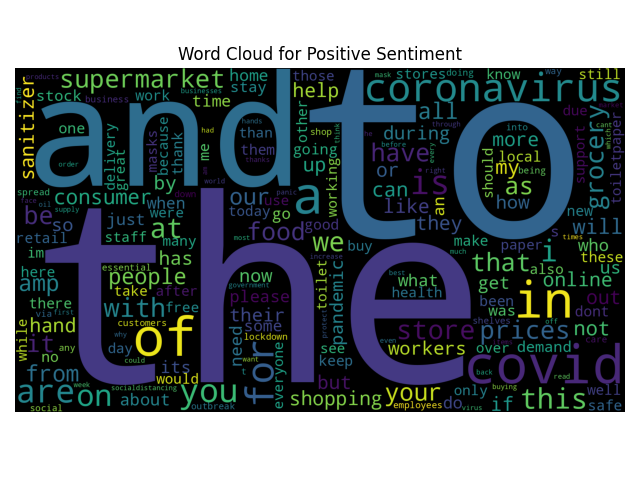
\includegraphics[width=0.8\textwidth]{Assignment 2/q1/wordcloud_Positive.png}
\end{figure}

\begin{figure}[H]
\centering
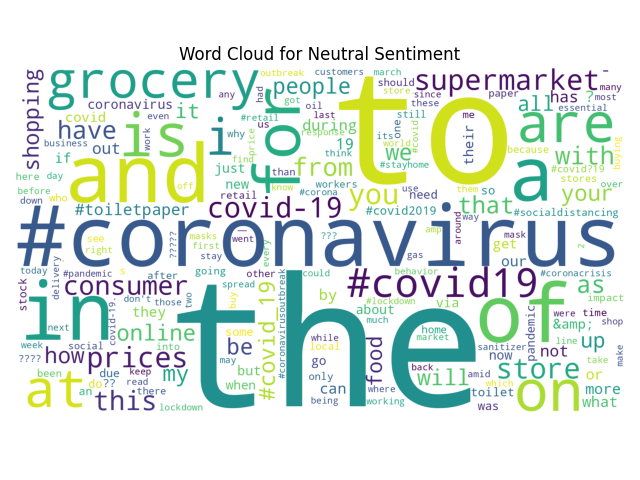
\includegraphics[width=0.8\textwidth]{Assignment 2/q1/wordcloud_Neutral.png}
\end{figure}

\begin{figure}[H]
\centering
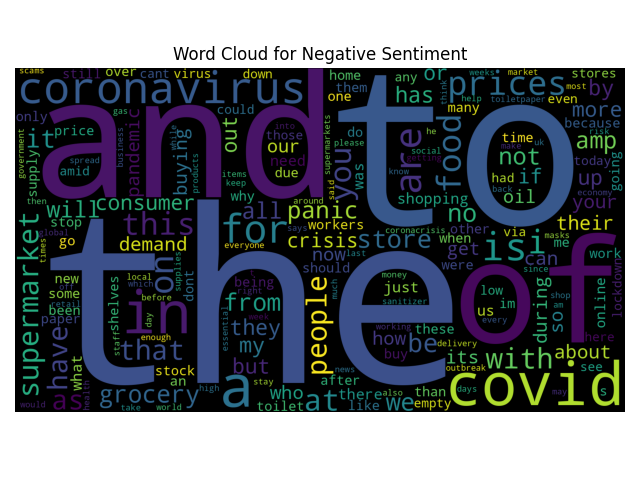
\includegraphics[width=0.8\textwidth]{Assignment 2/q1/wordcloud_Negative.png}
\end{figure}


\subsection{Random and Positive Baseline Accuracy}
\begin{itemize}
    \item Random:
    \begin{itemize}
        \item Training: 33.32 percent
        \item Validation: 32.82 percent
    \end{itemize}

    \item Positive:
    \begin{itemize}
        \item Training: 43.84 percent
        \item Validation: 43.85 percent
    \end{itemize}
\end{itemize}

For three classes, the accuracy of random guessing is:
\begin{equation}
\text{Accuracy} = \frac{1}{3}
\end{equation}

The accuracy when predicting all samples as positive is:
\begin{equation}
\text{Accuracy} = \frac{\text{Number of positive samples}}{\text{Total number of samples}}
\end{equation}

Comparing to the Naive Bayes Classifier I have created, as expected, it performs better than both Random and Positive Prediction.

\begin{table}[h]
    \centering
    \begin{tabular}{|l|c|c|}
    \hline
    \textbf{Method} & \textbf{Training Accuracy} & \textbf{Validation Accuracy} \\
    \hline
    Random & 33.32\% & 32.82\% \\
    \hline
    Positive & 43.84\% & 43.85\% \\
    \hline
    Naïve Bayes & 80.23\% & 69.96\% \\
    \hline
    \end{tabular}
    \caption{Comparison of different methods for text classification.}
    \label{tab:comparison}
\end{table}

The improvement of our Naïve Bayes classifier over:
    \begin{itemize}
        \item Random guessing is \( \approx 34.42\% \).
        \item Predicting all as "Positive" is \( \approx 23.90\% \).
    \end{itemize}



\subsection{Confusion Matrix}

\begin{table}[h]
    \centering
    \begin{tabular}{|c|c|c|c|}
    \hline
     & \textbf{Predicted Positive} & \textbf{Predicted Neutral} & \textbf{Predicted Negative} \\
    \hline
    \textbf{Actual Positive} & True Positives (TP) & False Neutral (FN) & False Negative (FN) \\
    \hline
    \textbf{Actual Neutral} & False Positive (FP) & True Neutrals (TN) & False Neutral (FN) \\
    \hline
    \textbf{Actual Negative} & False Positive (FP) & False Neutral (FN) & True Negatives (TN) \\
    \hline
    \end{tabular}
    \caption{Confusion Matrix Format}
    \label{tab:confusion_matrix}
\end{table}


\subsubsection{Naive Bayes}
\begin{center}
\textbf{Training Set}
\begin{center}
\begin{tabular}{|c|c|c|c|}
\hline
 & Positive & Negative & Neutral \\
\hline
Positive & 14770 & 1565 & 267 \\
\hline
Negative & 1699 & 12252 & 215 \\
\hline
Neutral & 2238 & 1500 & 3358 \\
\hline
\end{tabular}
\end{center}

\textbf{Validation Set}
\begin{center}
\begin{tabular}{|c|c|c|c|}
\hline
 & Positive & Negative & Neutral \\
\hline
Positive & 1196 & 226 & 22 \\
\hline
Negative & 254 & 952 & 26 \\
\hline
Neutral & 290 & 171 & 156 \\
\hline
\end{tabular}
\end{center}
\end{center}

\subsubsection{Random}
\begin{center}
\textbf{Training Set}
\begin{center}
\begin{tabular}{|c|c|c|c|}
\hline
 & Positive & Negative & Neutral \\
\hline
Positive & 5575 & 5528 & 5499 \\
\hline
Negative & 4834 & 4689 & 4643 \\
\hline
Neutral & 2407 & 2337 & 2352 \\
\hline
\end{tabular}
\end{center}

\textbf{Validation Set}
\begin{center}
\begin{tabular}{|c|c|c|c|}
\hline
 & Positive & Negative & Neutral \\
\hline
Positive & 465 & 505 & 474 \\
\hline
Negative & 401 & 427 & 404 \\
\hline
Neutral & 205 & 223 & 189 \\
\hline
\end{tabular}
\end{center}
\end{center}

\subsubsection{Positive}
\begin{center}
\textbf{Training Set}
\begin{center}
\begin{tabular}{|c|c|c|c|}
\hline
 & Positive & Negative & Neutral \\
\hline
Positive & 16602 & 0 & 0 \\
\hline
Negative & 14166 & 0 & 0 \\
\hline
Neutral & 7096 & 0 & 0 \\
\hline
\end{tabular}
\end{center}

\textbf{Validation Set}
\begin{center}
\begin{tabular}{|c|c|c|c|}
\hline
 & Positive & Negative & Neutral \\
\hline
Positive & 1444 & 0 & 0 \\
\hline
Negative & 1232 & 0 & 0 \\
\hline
Neutral & 617 & 0 & 0 \\
\hline
\end{tabular}
\end{center}
\end{center}


\begin{enumerate}
	\item Naive Bayes:

\begin{itemize}
		\item Training Set: The category with the highest value on the diagonal is Positive with 14770 correct predictions.
		\item Validation Set: The category with the highest value on the diagonal is Positive with 1196 correct predictions.
\end{itemize}

	\item Random:

\begin{itemize}
		\item Training Set: The category with the highest value on the diagonal is Positive with 5575 correct predictions.
		\item Validation Set: The category with the highest value on the diagonal is Positive with 465 correct predictions.
\end{itemize}

	\item Positive:

\begin{itemize}
		\item Training Set: The category with the highest value on the diagonal is Positive with 16602 correct predictions.
		\item Validation Set: The category with the highest value on the diagonal is Positive with 1444 correct predictions.
\end{itemize}

\end{enumerate}
The highest value on the diagonal entry indicates that this category was the most accurately predicted among the three. For all three methods (Naive Bayes, Random, and Positive), the "Positive" category has the highest number of correctly predicted instances. This means that the model is best at correctly identifying positive samples.




\subsection{Stopword Removal and Stemming}
\subsubsection{Data Transformation}
Stop Word removal is performed using the set of English stop words in the nltk corpus. Stemming is done using PorterStemmer from nltk.stem.

\subsubsection{Word Clouds}
\begin{figure}[H]
\centering
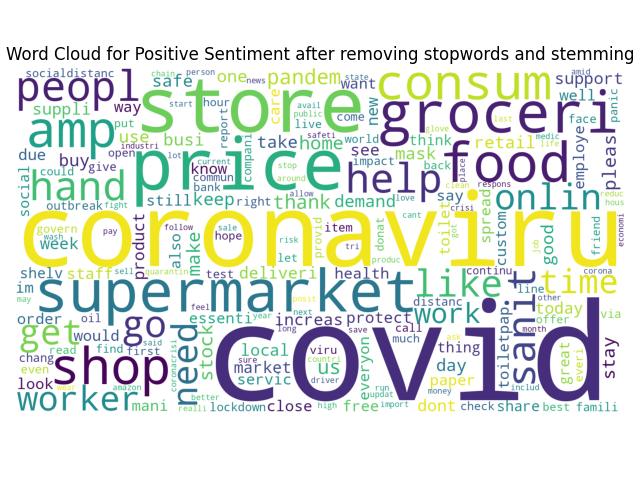
\includegraphics[width=0.8\textwidth]{Assignment 2/q1/wordcloud_Positive_stemming_and_removeStopwords.png}
\end{figure}

\begin{figure}[H]
\centering
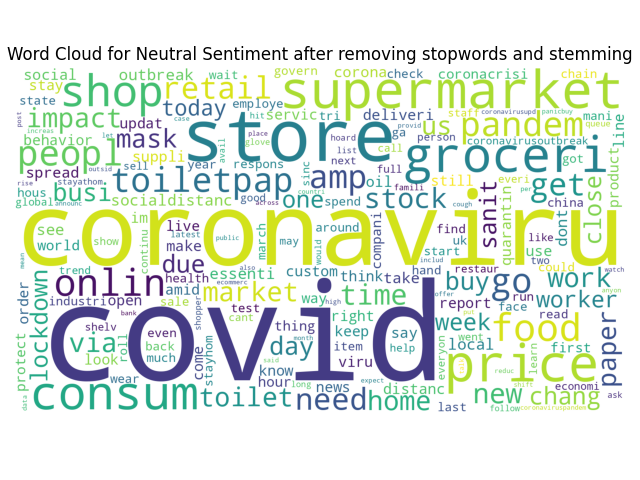
\includegraphics[width=0.8\textwidth]{Assignment 2/q1/wordcloud_Neutral_stemming_and_removeStopwords.png}
\end{figure}

\begin{figure}[H]
\centering
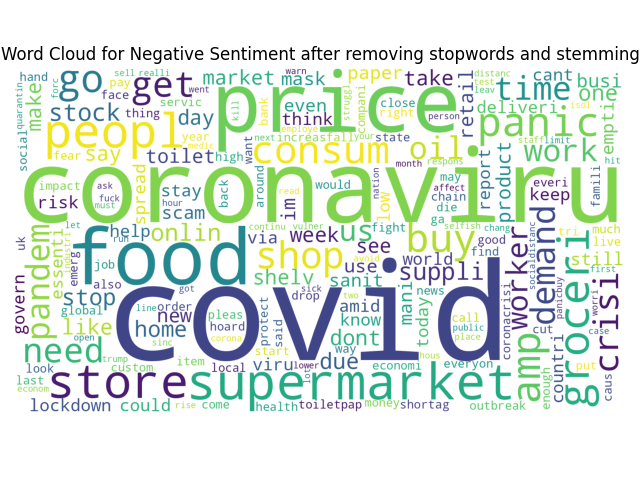
\includegraphics[width=0.8\textwidth]{Assignment 2/q1/wordcloud_Negative_stemming_and_removeStopwords.png}
\end{figure}

\subsubsection{Model Accuracy}
\begin{itemize}
    \item Training: 73.46 percent
    \item Validation: 65.65 percent
\end{itemize}

\subsubsection{Observations}
The wordclouds created after removing stop words and stemming more accurately represent the words with positive and negative sentiment. However, validation accuracy decreases slightly. 

Here are a few potential reasons for this reduction:

\begin{enumerate}
	\item Loss of Contextual Information: By removing stopwords, we may have inadvertently removed some contextual information from the tweets. In some cases, stopwords can provide valuable context. For instance, the phrase "not good" is negative, but if we remove the stopword "not", the sentiment could be misinterpreted.
	\item Over-Stemming: Stemming can sometimes be aggressive, merging words that should be distinct. This can lead to loss of valuable information. For example, the words "universe" and "university" might both be stemmed to "univers", even though they have very different meanings.
	\item Variability in Data: The nature of tweets is such that many words or phrases are used in a colloquial or slang manner. Some of these might be treated as stopwords or might get inappropriately stemmed, leading to loss of sentiment information.
	\item Model Simplicity: The Naïve Bayes classifier assumes that features (words, in this case) are independent given the class label. This is a strong assumption, especially for textual data where word order and context matter. The preprocessing might exacerbate the impact of this assumption by removing or altering words that provide context.
\end{enumerate}


\subsection{Feature Engineering}
\subsubsection{Using Bigrams}
\begin{itemize}
    \item Validation Accuracy: 66.17 percent
\end{itemize}

\subsubsection{Additional Feature: Number of Words}
Intuitively, the length of a tweet might give some information about its sentiment, with very short tweets possibly being more neutral or negative, while longer tweets might be more descriptive and positive.
\begin{itemize}
    \item Validation Accuracy: 66.32 percent
    \item Improvement of about 0.2 percent
\end{itemize}

\subsection{Domain Adaptation}
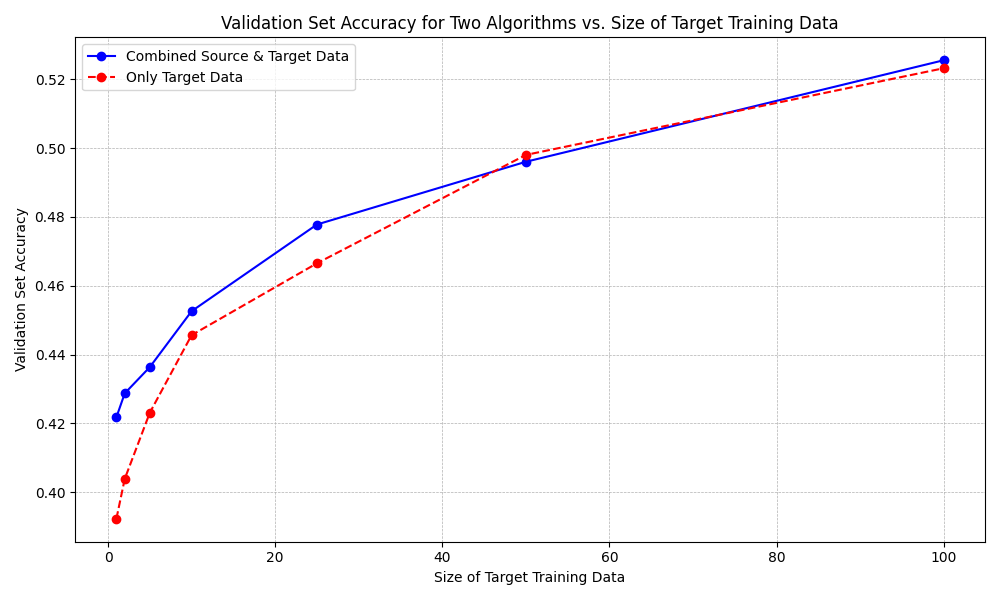
\includegraphics[width=\textwidth]{Assignment 2/q1/Domain adaptation validation_accuracies plot.png}

\subsubsection{Observations:}
\begin{itemize}
    \item For both algorithms, the validation accuracy increases as more target training data is added. This indicates that having more target domain data generally improves the model's performance on unseen target domain data.
    \item The first algorithm (combined source and target data) shows a more gradual increase in validation accuracy as the dataset size increases. By contrast, the second algorithm (only target data) starts with a lower validation accuracy for smaller datasets but catches up and eventually surpasses the first algorithm as the dataset size increases.
    \item The results indicate the value of domain adaptation. The first algorithm, which leverages data from the source domain, provides a head start in performance, especially when the target domain data is limited. As more target domain data becomes available, the advantage of using source domain data diminishes, and the second algorithm's performance surpasses the first.
\end{itemize}
In conclusion, these observations highlight the benefits of domain adaptation, especially when target domain data is limited. However, as more target domain data becomes available, the advantage of using only target domain data becomes apparent. The results also emphasize the importance of having a sufficiently large dataset to prevent overfitting and ensure better generalization to unseen data.

\section{Image Classification}
\subsection{Binary Classification}
\subsubsection{Using CVXOPT, Linear Kernel}
\text{Given the standard SVM dual formulation:}

\begin{align*}
\max_{\alpha} & \sum_{i=1}^{m} \alpha_i - \frac{1}{2} \sum_{i=1}^{m} \sum_{j=1}^{m} y^{(i)} y^{(j)} \alpha_i \alpha_j \langle x^{(i)}, x^{(j)} \rangle
\end{align*}

\text{subject to:}

\begin{align*}
0 & \leq \alpha_i \leq C, \\
\sum_{i=1}^{m} \alpha_i y^{(i)} & = 0
\end{align*}

\text{The CVXOPT standard quadratic problem format is:}

\begin{align*}
\min_{\alpha} & \frac{1}{2} \alpha^T P \alpha + q^T \alpha
\end{align*}

\text{subject to:}

\begin{align*}
G\alpha & \leq h, \\
A\alpha & = b
\end{align*}

\text{To put the SVM dual in this form:}

\begin{itemize}
\item \( P \) is an \( m \times m \) matrix where \( P_{ij} = y^{(i)} y^{(j)} \langle x^{(i)}, x^{(j)} \rangle \)
\item \( q \) is an \( m \) sized column vector with all elements being -1.
\item \( G \) is a \( 2m \times m \) matrix constructed such that it considers both \( \alpha_i \geq 0 \) and \( \alpha_i \leq C \).
\item \( h \) is a \( 2m \) sized vector with first \( m \) elements being 0 and next \( m \) elements being \( C \).
\item \( A \) is a \( 1 \times m \) row vector with elements as the labels \( y^{(i)} \).
\item \( b \) is a scalar 0.
\end{itemize}


\[ w = \sum_{i=1}^{m} \alpha_i y^{(i)} x^{(i)} \]


For a chosen support vector \( x_s \): \\
\[ b = y_s - \sum_{i=1}^{m} \alpha_i y^{(i)} \langle x^{(i)}, x_s \rangle \]
Ensure \( 0 < \alpha_s < C \) for the chosen \( x_s \).

\[ \text{prediction} = \text{sign}(\langle w, x \rangle + b) \]

\paragraph{Results:}
\begin{itemize}
    \item Number of Support Vectors Obtained: 2383
    \item Percentage of training samples constituting support vectors: 50.06 percent
    \item Intercept (b)= 1.041890005986661
    \item The Validation accuracy came to be 77.5 percent.
    \item 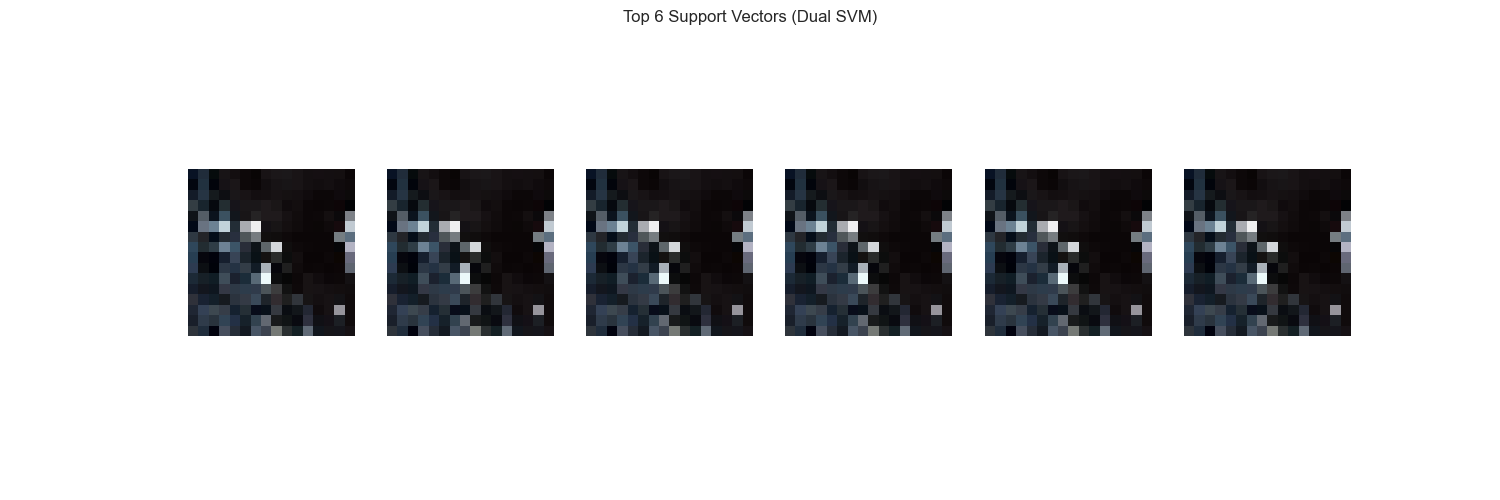
\includegraphics[width=\textwidth]{Assignment 2/q2/top_6_support_vectors_dual cvxopt linear.png}
    \item 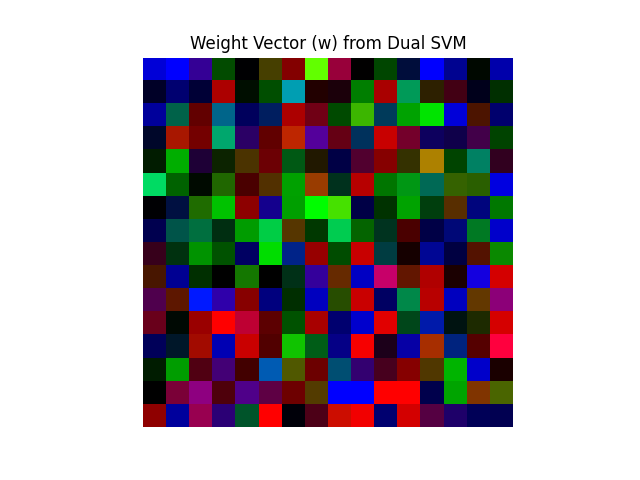
\includegraphics[width=\textwidth]{Assignment 2/q2/weight_vector_dual cvxopt linear.png}
\end{itemize}

\subsubsection{Using CVXOPT, Gaussian Kernel}

The Gaussian (or Radial Basis Function - RBF) kernel between two points \( x \) and \( z \) is defined as:
\[
K(x, z) = \exp(-\gamma \|x - z\|^2)
\]
where \( \gamma \) is a parameter that controls the width of the Gaussian function.

section*{SVM Dual Formulation with Gaussian Kernel}

The dual formulation of the SVM optimization problem with the Gaussian kernel is:
\begin{align*}
\text{maximize} \quad & \sum_{i=1}^{m} \alpha_i - \frac{1}{2} \sum_{i=1}^{m} \sum_{j=1}^{m} \alpha_i \alpha_j y^{(i)} y^{(j)} K(x^{(i)}, x^{(j)}) \\
\text{subject to} \quad & 0 \leq \alpha_i \leq C \\
& \sum_{i=1}^{m} \alpha_i y^{(i)} = 0
\end{align*}
where:
\begin{itemize}
    \item \( \alpha_i \) are the dual variables
    \item \( y^{(i)} \) are the labels, taking values in \{ -1, 1 \}
    \item \( K(x^{(i)}, x^{(j)}) \) is the Gaussian kernel between points \( x^{(i)} \) and \( x^{(j)} \)
    \item \( C \) is a regularization parameter
\end{itemize}

CVXOPT solves the quadratic programming problem in the following standard form:
\begin{align*}
\text{minimize} \quad & \frac{1}{2} \alpha^T P \alpha + q^T \alpha \\
\text{subject to} \quad & G\alpha \leq h \\
& A\alpha = b
\end{align*}
To express the SVM dual in this form:
\begin{itemize}
    \item \( P \) is an \( m \times m \) matrix with elements \( P_{ij} = y^{(i)} y^{(j)} K(x^{(i)}, x^{(j)}) \)
    \item \( q \) is an \( m \)-sized column vector with all elements being -1
    \item \( G \) is a \( 2m \times m \) matrix constructed such that it considers both \( \alpha_i \geq 0 \) and \( \alpha_i \leq C \)
    \item \( h \) is a \( 2m \)-sized vector with the first \( m \) elements being 0 and the next \( m \) elements being \( C \)
    \item \( A \) is a \( 1 \times m \) row vector with elements as the labels \( y^{(i)} \)
    \item \( b \) is a scalar 0
\end{itemize}

\paragraph{Results:}

\begin{itemize}
    \item Number of support vectors: 3058
    \item Validation Accuracy: 75.5 precent
\end{itemize}



\subsubsection{Using scikit-learn SVM function, Linear Kernel}

\paragraph{Results:}
\begin{itemize}
    \item Number of Support Vectors Obtained: 2371
    \item Percentage of training samples constituting support vectors: 49.81 percent
    \item Intercept (b)= 1.06989668
    \item The Validation accuracy came to be 78 percent.
    \item 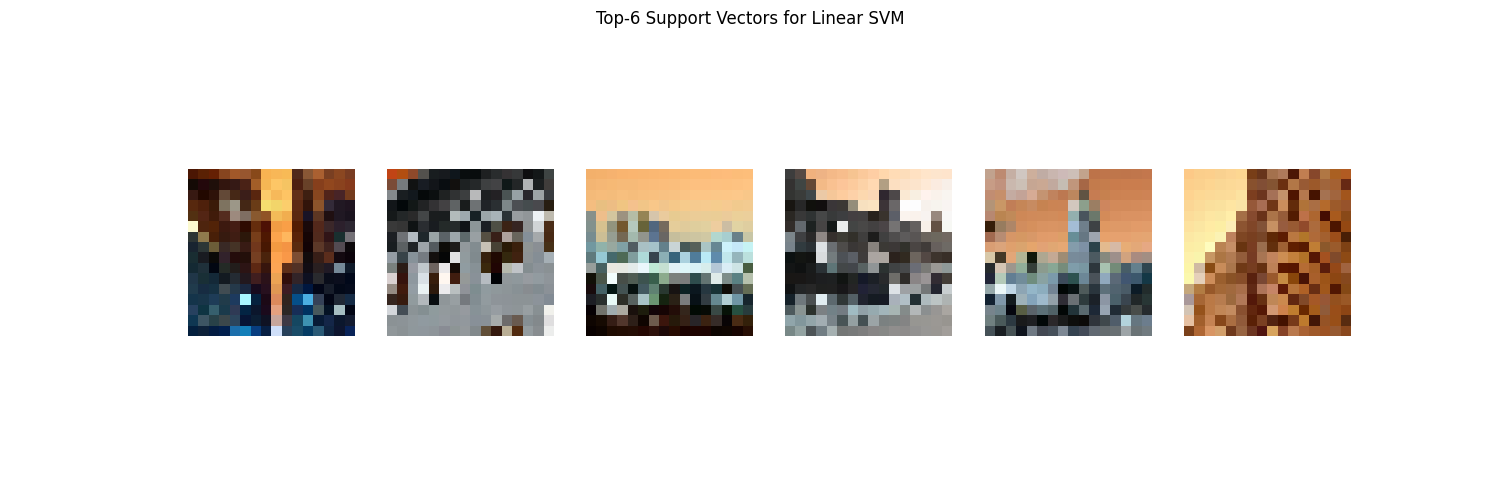
\includegraphics[width=\textwidth]{Assignment 2/q2/top_6_support_vectors_linear libsvm linear.png}
    \item 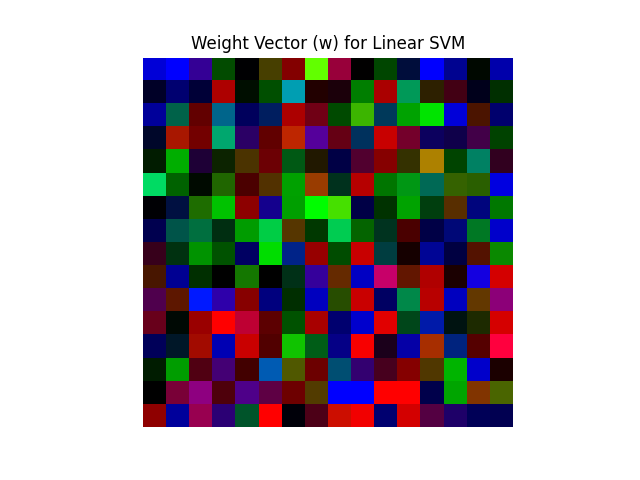
\includegraphics[width=\textwidth]{Assignment 2/q2/weight_vector_linear libsvm linear.png}
\end{itemize}

\subsubsection{Using scikit-learn SVM function, Gaussian(RBF) Kernel}
\paragraph{Results:}
\begin{itemize}
    \item Number of Support Vectors Obtained: 3054
    \item Percentage of training samples constituting support vectors: 64.16 percent
    \item The Validation accuracy came to be 75.25 percent.
    \item 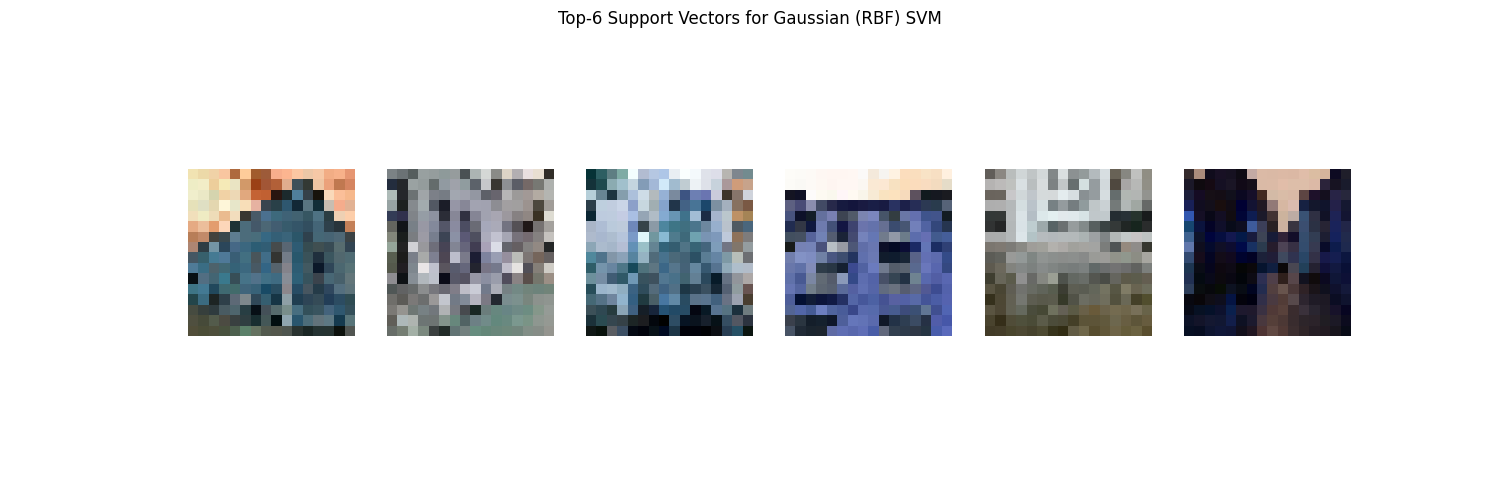
\includegraphics[width=\textwidth]{Assignment 2/q2/top_6_support_vectors_rbf libsvm rbf.png}
\end{itemize}

\subsubsection{Comparison of b and Support Vectors}
\paragraph{For Gaussian Kernel}
\begin{itemize}
    \item b found using cvxopt = -1.06832676477997
    \item b found using libsvm = -1.0622098653371628
    \item The bs obtained are approximately equal
    \item 3054 support vectors match
\end{itemize}

\paragraph{For Linear Kernel}
\begin{itemize}
    \item b found using cvxopt = 1.041890005986661
    \item b found using libsvm = 1.06989668
    \item 2371 support vectors match
    \item 383 entries in w are not within a margin of 1e-5 
\end{itemize}

\paragraph{Between Linear and Gaussian Kernel}
\begin{itemize}
    \item 2206 support vectors match when using cvxopt
    \item 2190 support vectors match when using libsvm
\end{itemize}

\subsection{Multi-Class Image Classification}
\subsubsection{One-vs-One Multi-Class SVM using CVXOPT}
\begin{itemize}
    \item Validation Accuracy: 56 percent
\end{itemize}

\subsubsection{Using scikit-learn SVM function}
\begin{itemize}
    \item Validation Accuracy: 55.91 percent
    \item The validation accuracy is almost similar to what was obtained using CVXOPT
    \item The training time for LIBSVM was considerably smaller compared to CVXOPT(2 minutes vs 17 minutes)
\end{itemize}

\subsubsection{Confusion Matrix and Observations}
\paragraph{For CVXOPT:}
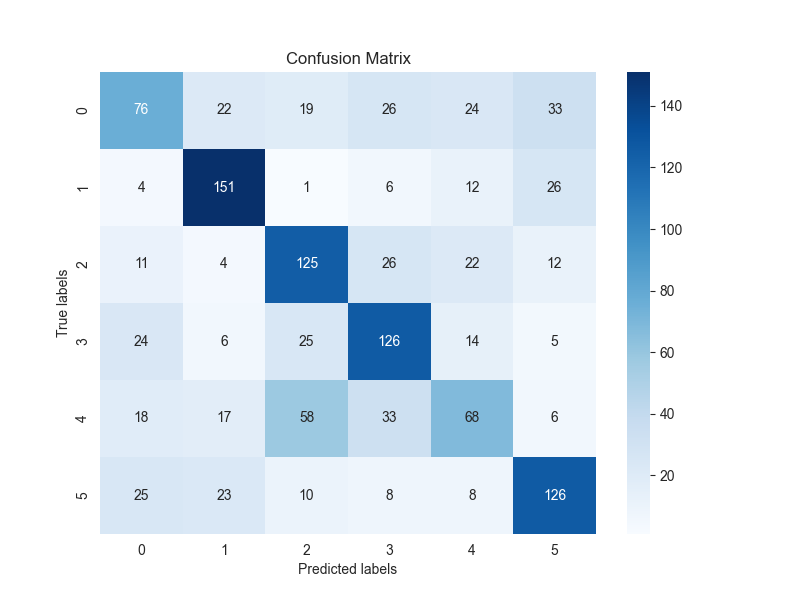
\includegraphics[width=0.6\textwidth]{Assignment 2/q2/confusion_matrix cvxopt.png}


\paragraph{For LIBSVM:}

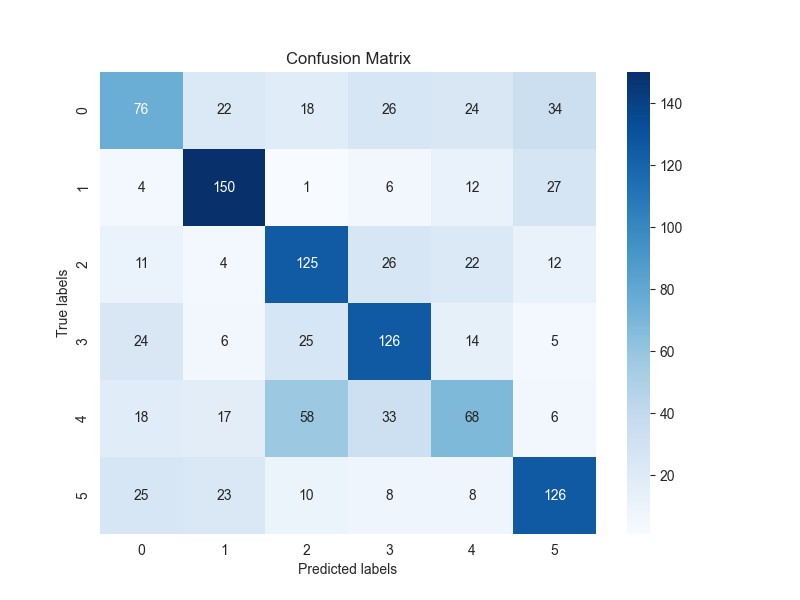
\includegraphics[width=0.6\textwidth]{Assignment 2/q2/confusion_matrix libsvm.png}
\begin{itemize}
    \item We can see that 58 examples of class 4 are predicted as class 2, this is the highest number among classes being misclassified
\end{itemize}
Some misclassified images:


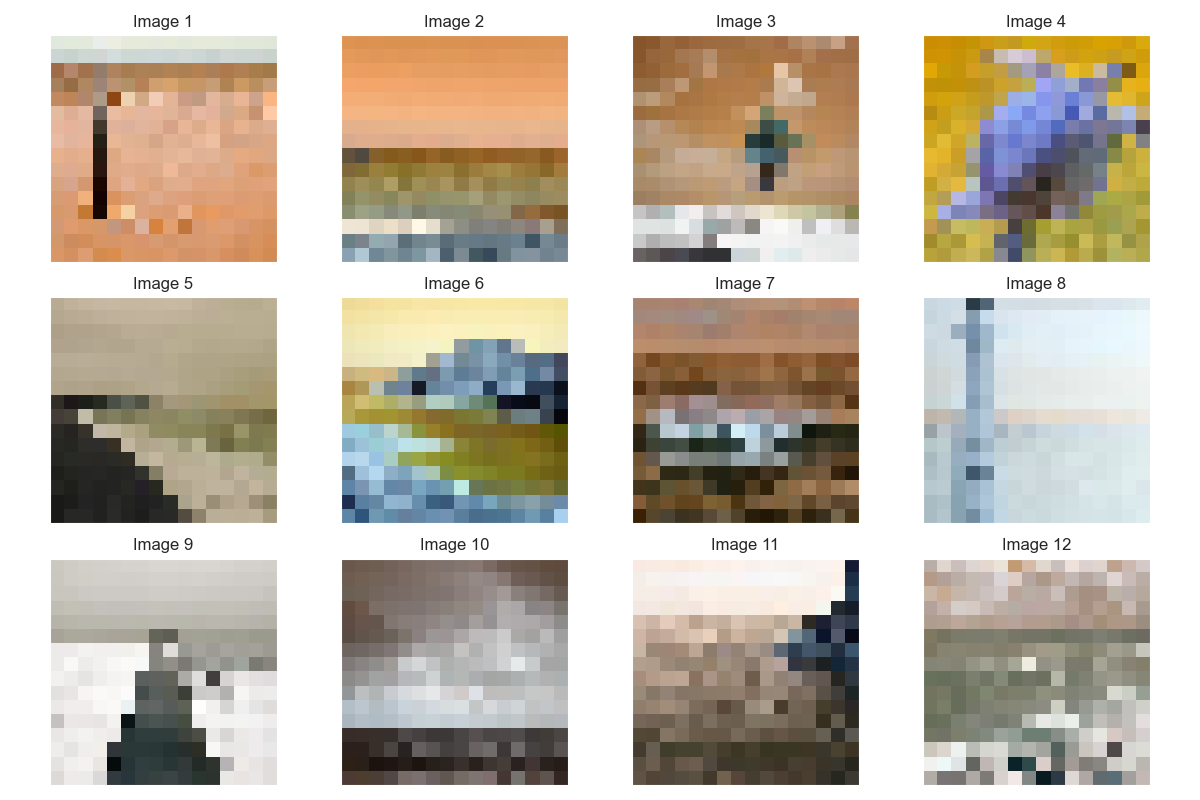
\includegraphics[width=0.7\textwidth]{Assignment 2/q2/misclassified_4_2.png}


This misclassification makes sense. Th mapping for Intel image classification dataset is 'buildings' - 0,
'forest' - 1,
'glacier' - 2,
'mountain' - 3,
'sea' - 4,
'street' - 5. Classifying into glacier and sea is a more intricate task compared to others, as they are somewhat similar in images.


\subsubsection{Validation and Cross-Validation}
% Write your answers for part 2(d) here.
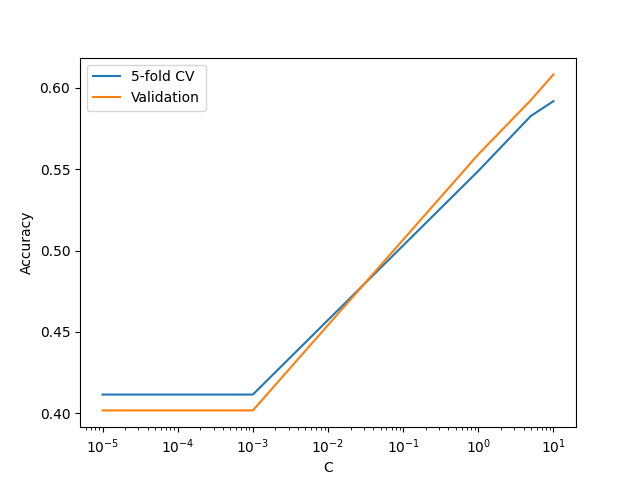
\includegraphics[width=\textwidth]{Assignment 2/q2/cross_validation_mult real.png}

As is evident from the graph, higher values of C are better, thus 10 is the best value. 
The model achieves the highest cross-validation accuracy of 59.03 with C=10. The validation accuracy for this setting is 60.83.

It has the highest validation and cross validation accuracy. 

\( C = 1 \times 10^{-5} \) and \( C = 0.001 \) both lead to poor performance with a CV accuracy of \( 15.81\% \) and a validation accuracy of \( 40.17\% \). This might indicate underfitting.

\( C = 1 \) has a CV accuracy of \( 54.85\% \) and a validation accuracy of \( 55.83\% \).

\( C = 5 \) results in a CV accuracy of \( 57.87\% \) and a validation accuracy of \( 59.25\% \).

As mentioned, \( C = 10 \) gives the best results.

There's an upward trend in performance as \( C \) increases from \( 1 \times 10^{-5} \) to \( 10 \). However, after \( C = 10 \), the performance starts decreasing, suggesting that \( C = 10 \) might be an optimal value in this range.

Very low values of \( C \) (like \( 1 \times 10^{-5} \) and \( 0.001 \)) lead to poor performance, suggesting potential underfitting. The model might be too regularized and fails to capture the underlying patterns in the data.


Note that the cross validation accuracy for lower vlaues of C such as C=1e-5 is very less, it is almost the same as a random classifier. This is because the number of elements of each class might not be same in each of the folds. If the folds are kept uniform, we get higher cross validation accuracy for lower values of C(around 40 percent). This is called Stratified KFold.
\end{document}
